\documentclass[12pt,a4paper]{scrartcl}

\usepackage[utf8]{inputenc}
\usepackage[T1]{fontenc}
\usepackage[british,UKenglish,USenglish,american]{babel}

\usepackage[pdftex]{graphicx}
\usepackage{latexsym}
\usepackage{amsmath,amssymb,amsthm}
\allowdisplaybreaks
\usepackage{dsfont}
\usepackage{pifont}
\usepackage{nicefrac}
\usepackage{textcomp}
\usepackage{enumitem}
\usepackage{lmodern}
\usepackage{bbm}

% Abstand obere Blattkante zur Kopfzeile ist 2.54cm - 15mm
\setlength{\topmargin}{-15mm}	   
                  
%\numberwithin{equation}{section} 
\numberwithin{equation}{subsection}

\newcommand{\C}{\mathbb{C}} % komplexe
\newcommand{\R}{\mathbb{R}} % reelle
\newcommand{\Q}{\mathbb{Q}} % rationale
\newcommand{\Z}{\mathbb{Z}} % ganze
\newcommand{\N}{\mathbb{N}} % natuerliche
\newcommand{\PP}{\mathbb{P}} % Probability
\newcommand{\E}{\mathcal{E}} % big Epsilon
\newcommand{\K}{\mathcal{K}}
\newcommand{\1}{\mathbbm{1}}

\numberwithin{equation}{section}

\theoremstyle{definition}
\newtheorem{example}{Example}[subsection]
\newtheorem{theorem}{Theorem}[subsection]
\newtheorem{corollary}{Corollary}[subsection]
\newtheorem{lemma}{Lemma}[subsection]
\newtheorem{definition}{Definition}[subsection]
\newtheorem{proposition}{Proposition}[subsection]
\newtheorem{algorithm}{Algorithm}[subsection]
\newtheorem{prop}{Proposition}[subsection]
\newtheorem{remark}{Remark}[subsection]
\newtheorem{pro}{Proof}
\newtheorem{comment}{Comment}[subsection]


\begin{document}
	\pagestyle{empty}

\begin{titlepage}

	
\includegraphics[scale=0.45]{kit-logo.jpg} 
    \vspace*{2cm} 
\begin{center} \large 
    
   Trash
\end{center}
\end{titlepage}

\newpage

\newpage
\phantom \\
\newpage

\tableofcontents %Inhaltsverzeichnis

 	\pagestyle{headings}

\setcounter{page}{1}

\newpage
\section{Einleitung}
External DLA beschreibt einen stochastischen Prozess, welcher zumindest in ähnlicher Form in natürlichen Prozessen beobachtbar ist. Er ähnelt zum Beispiel der fraktalen Gestalt eines sich kreisförmig ausbreitenden Risses einer Glasscheibe, oder eines Risses eines Kristallfluids wie in LCD Displays in alten Autoradios (siehe Fotos). Er kann auch in Schneeflocken oder in elektrostatischen Anhaftungen an Metallen beobachtet werden. Die Formalisierung solcher Prozesse ist sehr aktuell und die sehr konstruktive Definition erlaubten bisher nur mühsame Folgerungen über Struktur und Verhalten des Prozesses. Wir werden uns Modelle auf $\mathbb{Z}^2$, sowie auf anderen Graphen, darunter auch fraktale Graphen, anschauen, und außerdem versuchen, eine Approximation der bisherigen Definition zu finden, die grundsätzlich handlicher ist und auf einfachere Weise zu Erkenntnissen führt. Wir werden außerdem diese Arbeit mit einigen Python Simulationen begleiten. Der Code ist frei verfügbar auf Github. \\
\\

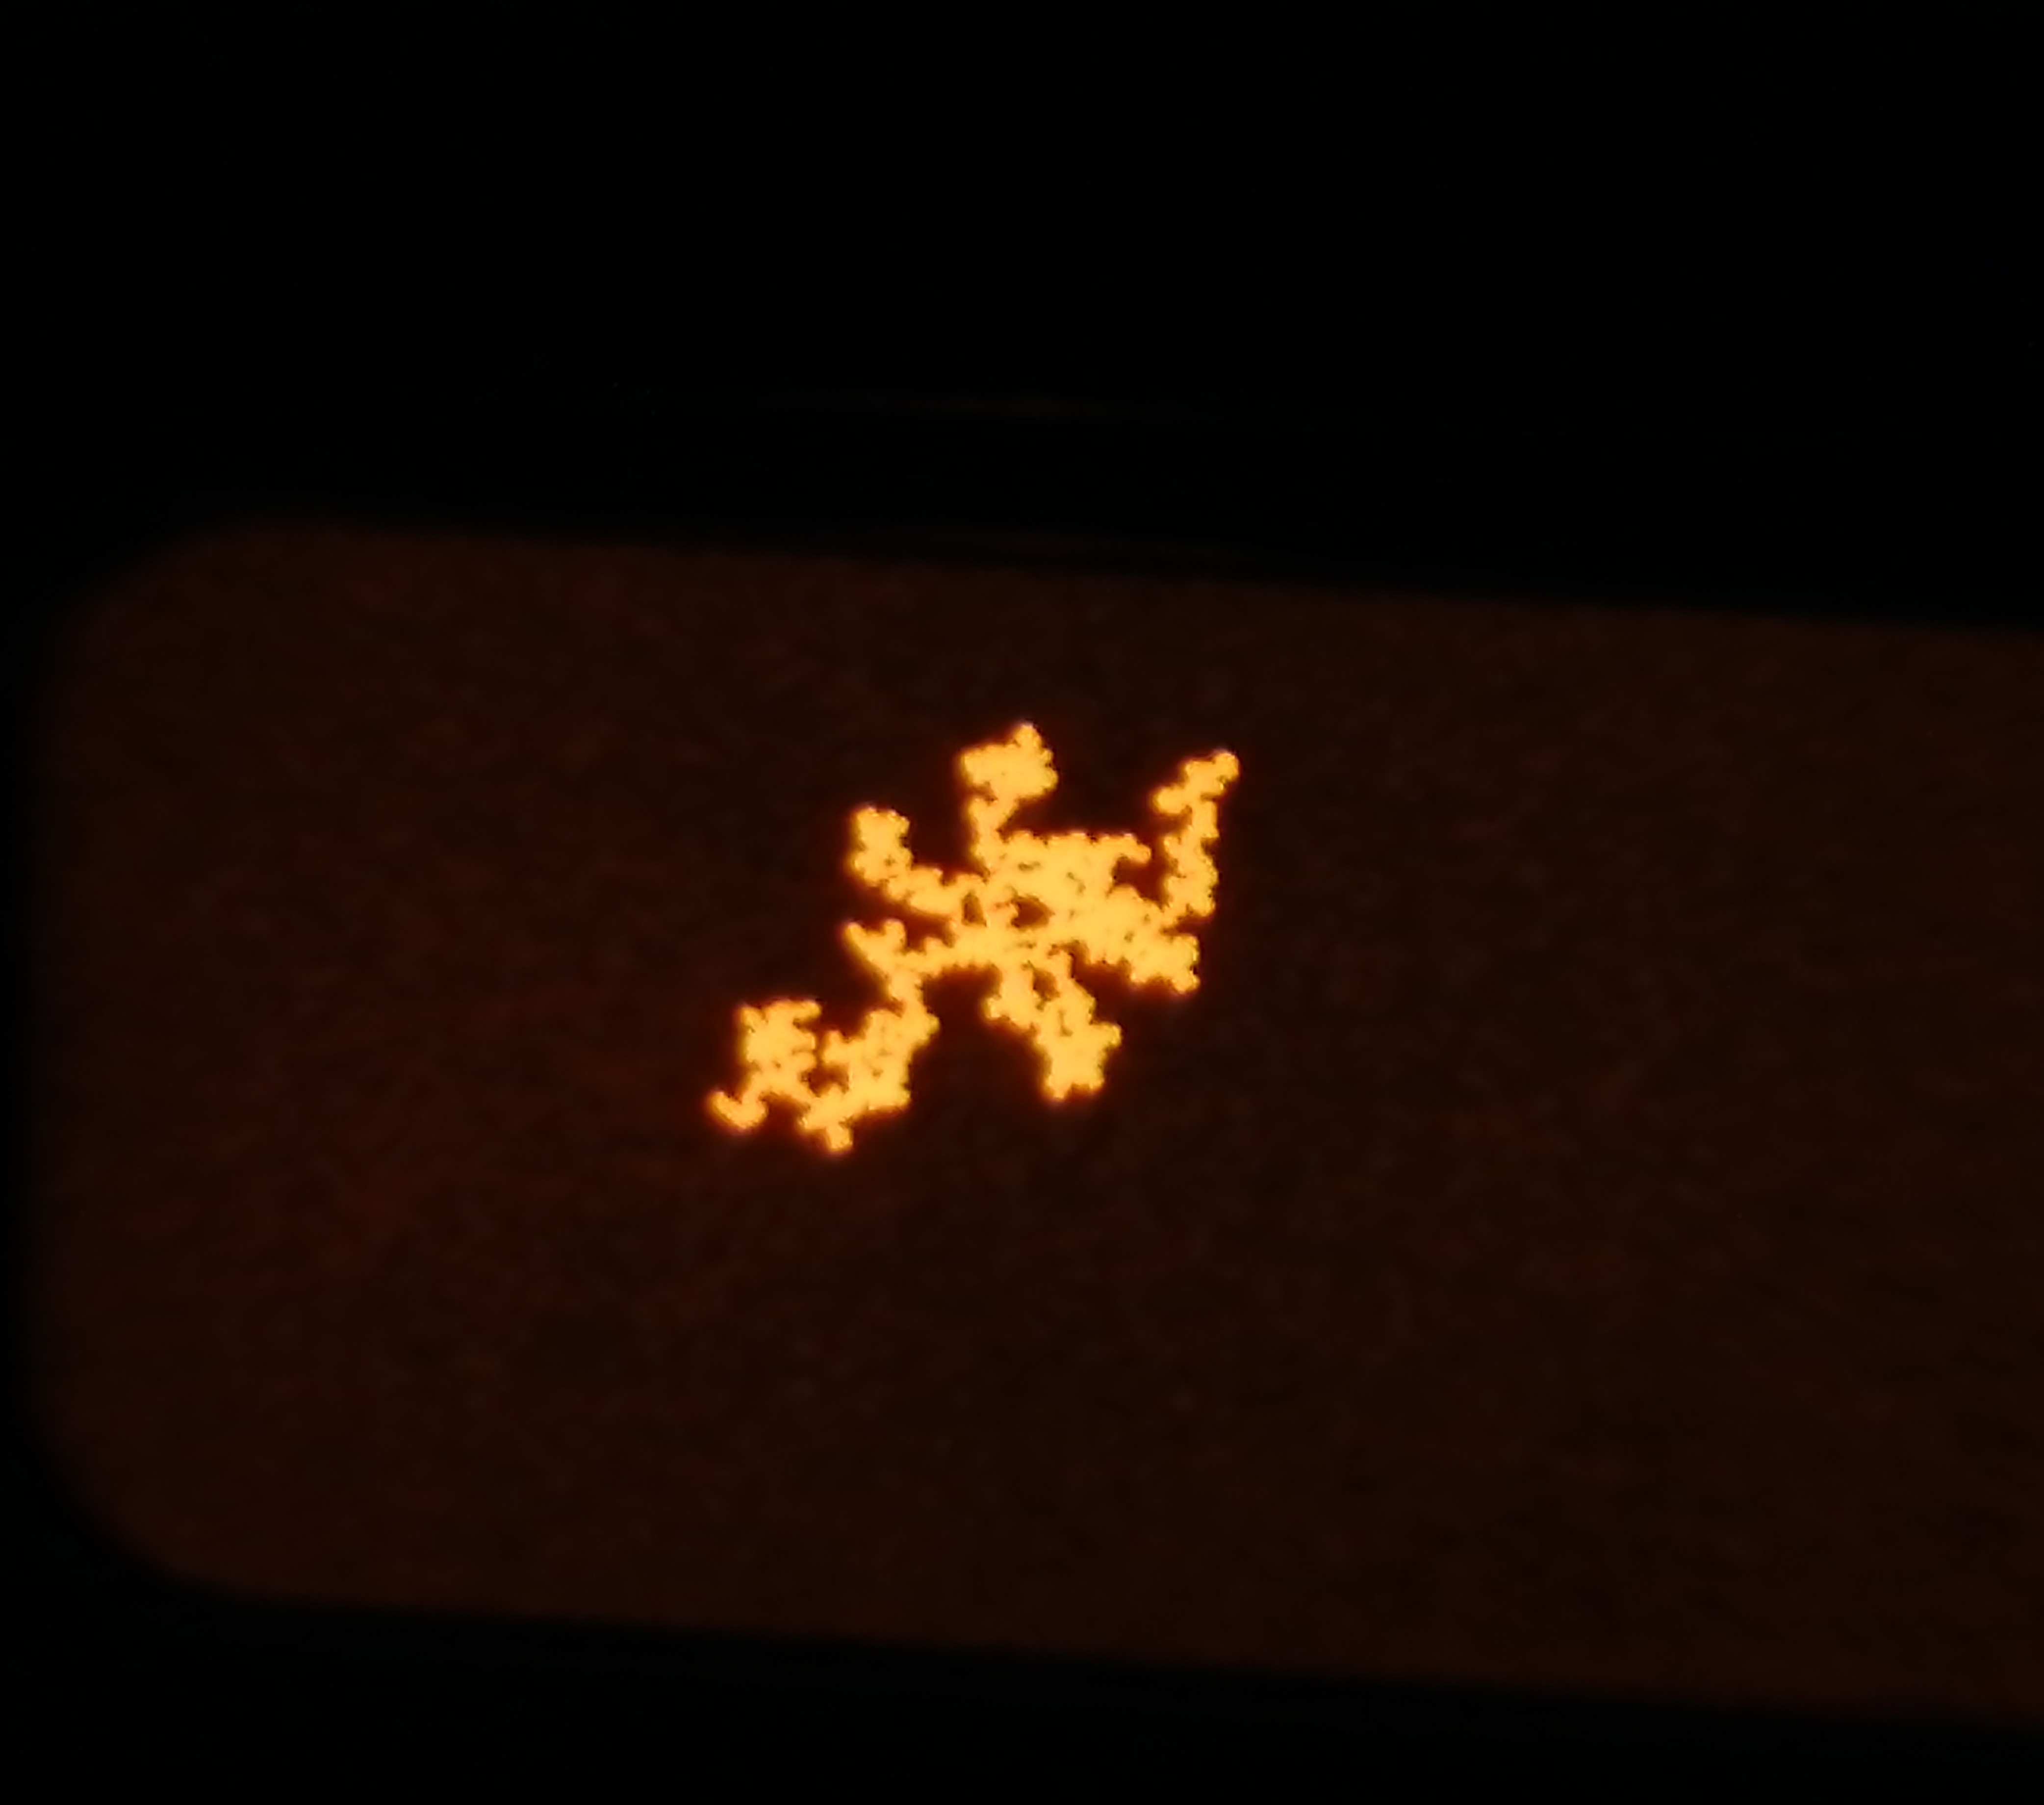
\includegraphics[scale=0.04]{display.jpg} 
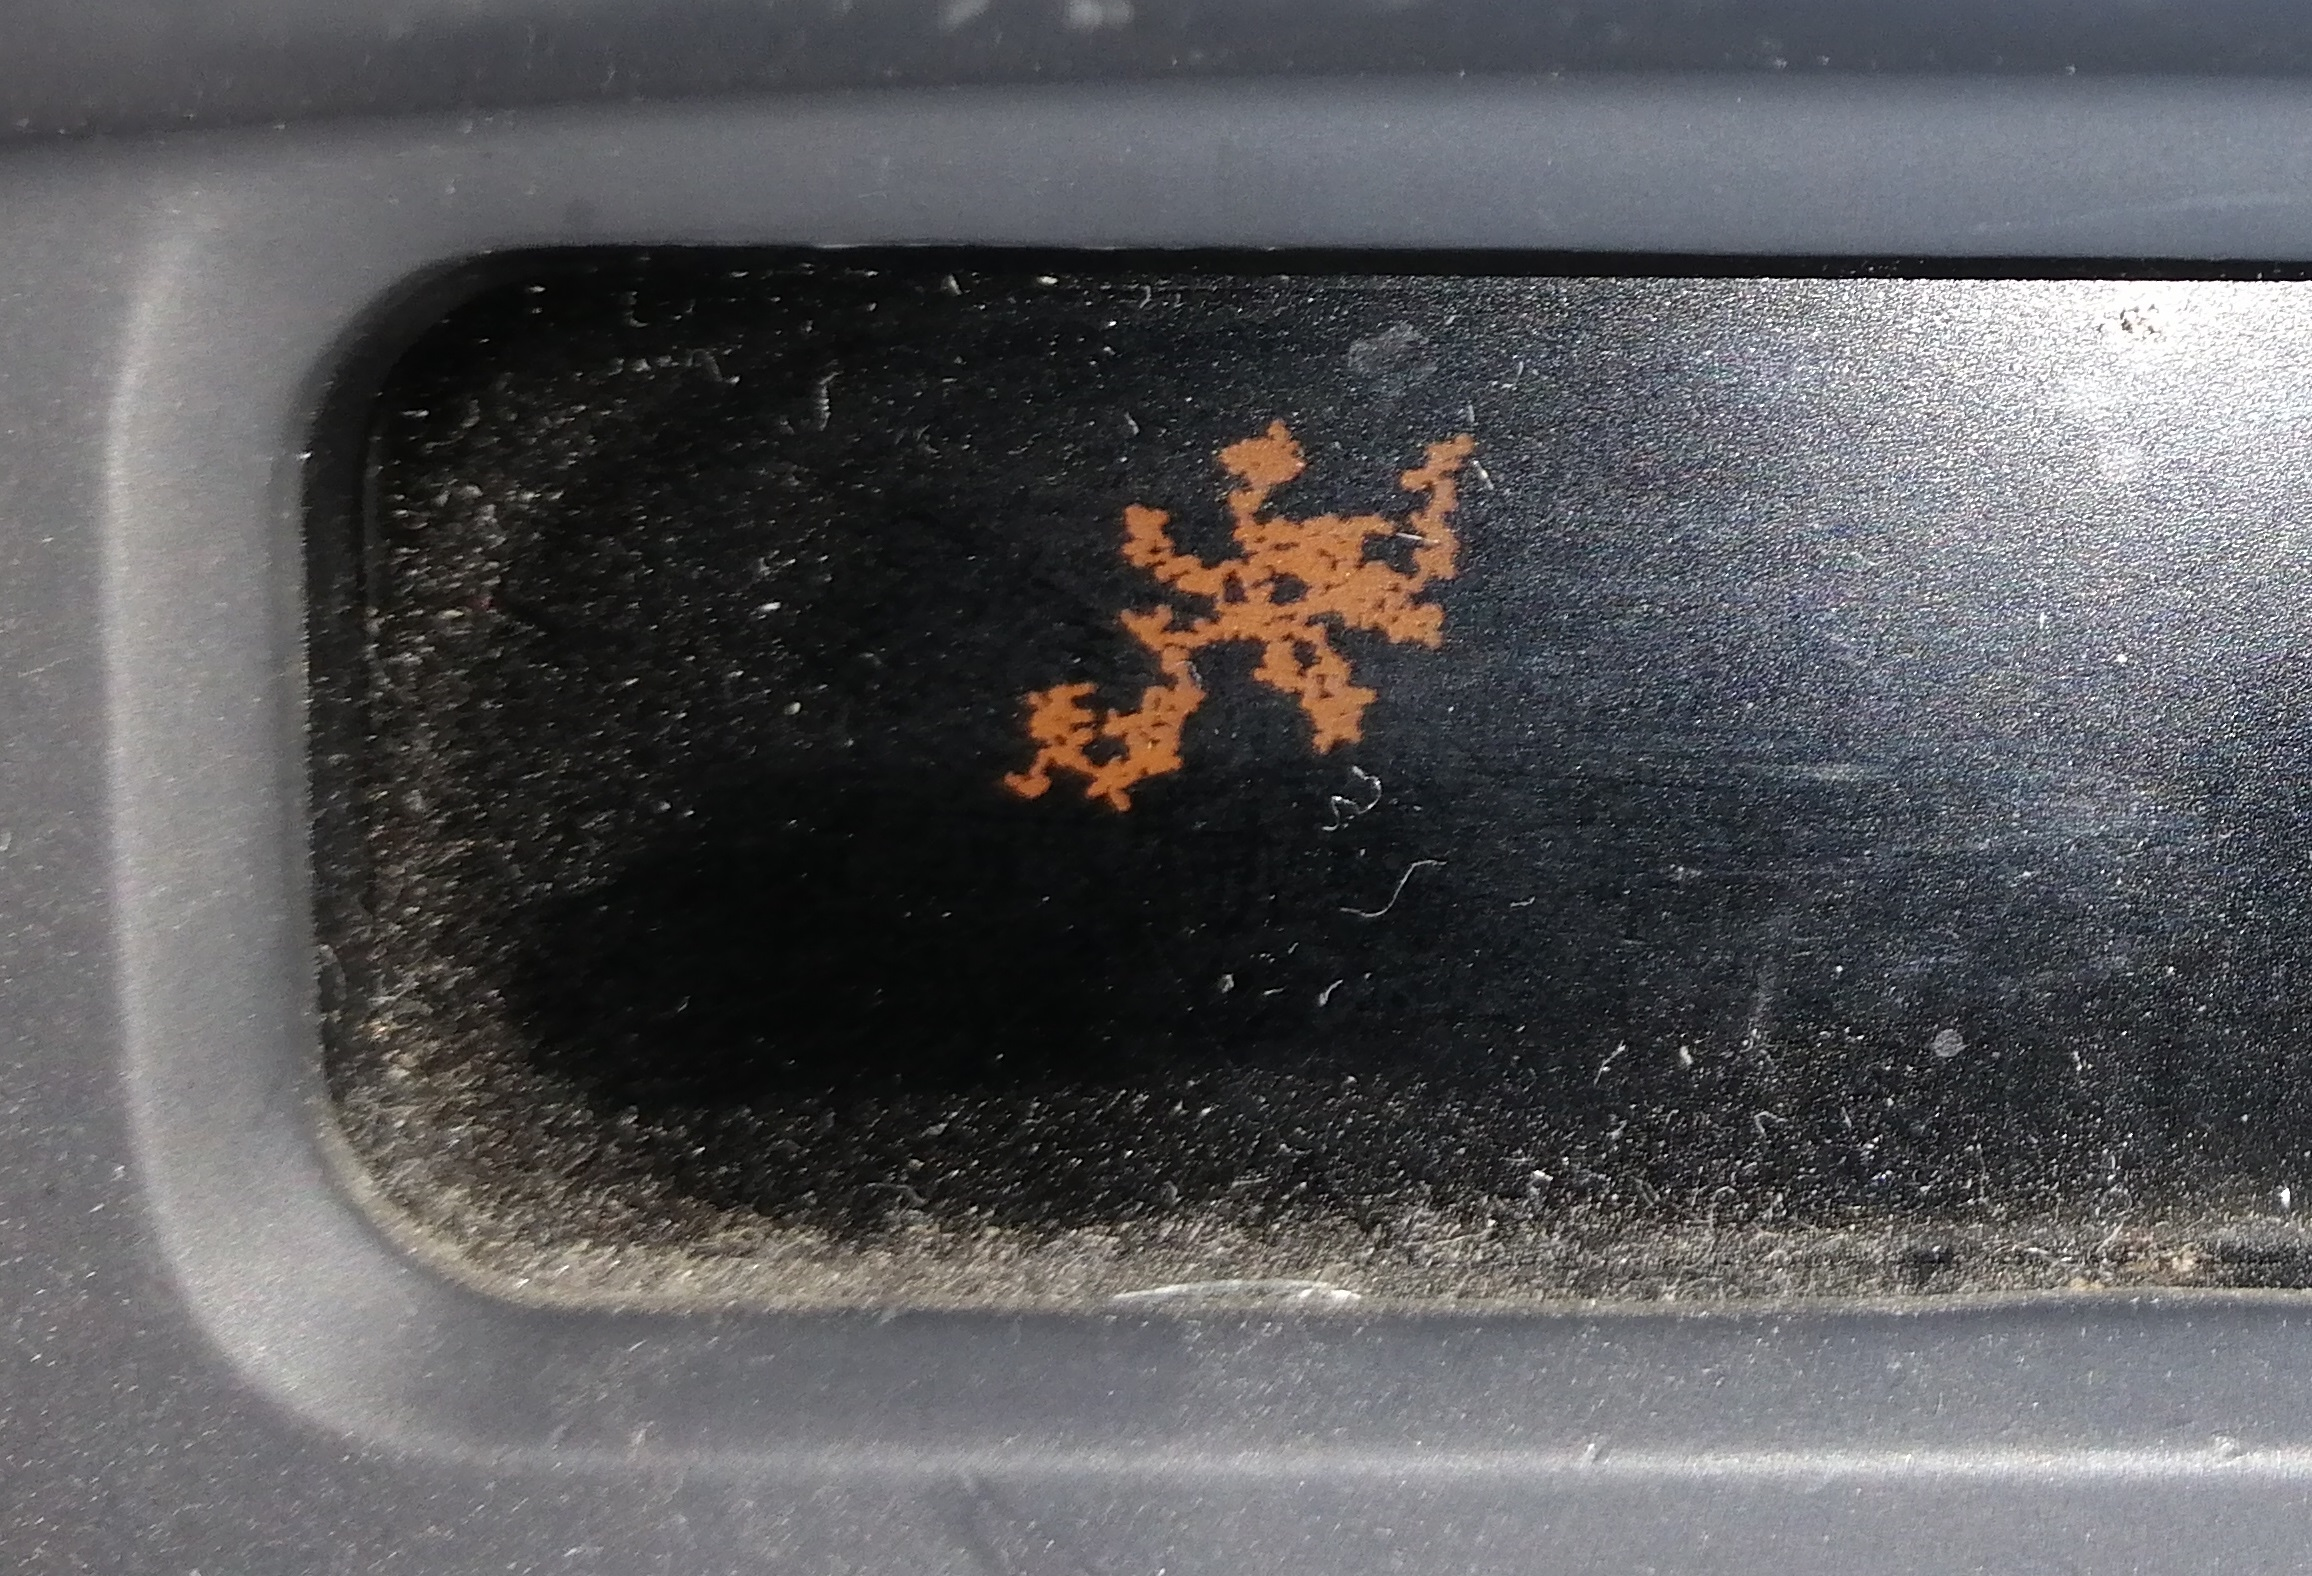
\includegraphics[scale=0.091]{display2.jpg} 

\newpage
\section{harmonic measure}
For the following we are interested in letting start the random walk "from infinity". Thus we are looking for someting like $\lim_{|x|\to\infty} h_A(x,y)$ for $y\in A$. This is solved the following way. Define the $\mathit{escape\ probability}$ from $A$  
\begin{flalign*}
e_A(x) := \1\{x\in A\}\PP(T_A^+=\infty), \quad x\in \Z^2
\end{flalign*}
and the $\mathit{capacity}$ of $A$
\begin{flalign*}
cap(A) := \sum_{x\in \Z^2} e_A(x). 
\end{flalign*}
Note that this sum is finite since $A$ is finite. Now we can define the $\mathit{harmonic\ measure}$ (from infinity) of $A$ as
\begin{flalign*}
h_A(x) := \frac{e_A(x)}{cap(A)}, \quad x\in \Z^2.
\end{flalign*}
The idea here is to use the symmetry of random walks and to not look the probability of coming from infinity to hit $A$, but actually starting in $A$ and stating the probability to escape $A$, which means to never hit $A$ again and therefore necessarily move away to infinity. We finally define the harmonic measure $h=(h_A)_{A\in \mathcal{P}_f}$.

\begin{lemma}
	Does something like $\lim_{|x|\to\infty} h_A(x,y)$ exist and is it equal to $h_A(y)$ for all $y\in A$?
\end{lemma}

\newpage
\section{A naive attempt}

We will look closer at the thought of the last Remark and find a reason, why this way of choosing a random line intersecting $K_0\in\K^2$ is maybe not the best idea. 

\begin{definition}
	Let $\gamma \sim \mathcal{U}([0,\pi))$ and for $\alpha \in [0,\pi)$ define $y_\alpha \sim \mathcal{U}(M_\alpha(K_0))$ where 
	\begin{align*}
		M_\alpha(K):= \begin{cases}
		\{h\in \mathbb{R}\ |\ L_{\tbinom{0}{h}, \tbinom{1}{0}} \cap K \neq \emptyset\},\quad \text{ if } \alpha = 0\\
		\{h\in \mathbb{R}\ |\ L_{\tbinom{h}{0}, \tbinom{cos(\alpha)}{sin(\alpha)}} \cap K \neq \emptyset\},\quad \text{ if } \alpha\in (0,\pi).
		\end{cases} 
	\end{align*}
	For $K\in \K^2$ define 

	\begin{flalign*}
		\nu_{K_0}(K) := \int_{[0,\pi)} \mathbb{P}_{y_\alpha}(M_\alpha(K\cap K_0)) \mathbb{P}_\gamma(d\alpha).
	\end{flalign*}
	Interpretation: $\nu_{K_0}(K)$ is the probability that a random line which intersects with $K_0$ also intersects with $K_0 \cap K$. \\
	Conjecture: $\nu_{K_0}(K) = \frac{\mu_1(K\cap K_0)}{\mu_1(K_0)}$ for $K,K_0\in \K^2$ ($\mu_1$  Gradenmaß).
\end{definition}

\begin{remark}
	Note that $	M_\alpha(K) \in\K^1$ for all $K\in \K^2$ and $\alpha\in [0,\pi)$ (Proof). Proof rotation symmetry.
\end{remark}

\begin{example}
	Let $0<r<R$ and $K_0 := B_R$ and analogously $K:=B_r$. Note that $K,K_0\in \K^2$ and $K\subset K_0$. Then by trigonometry we get 
	\begin{flalign*}
		M_\alpha(K_0) = \begin{cases}
			[-R,R],\quad \text{ if } \alpha=0,\\
			[-\frac{R}{sin(\alpha)}, \frac{R}{sin(\alpha)}],\quad \text{ if } \alpha\in (0,\pi)
		\end{cases}
	\end{flalign*} 
	and analogously $M_\alpha(K)$. Finally we get
	\begin{flalign*}
		\nu_{K_0}(K) &= \int_{[0,\pi)} \PP_{y_\alpha}(M_\alpha(K\cap \K_0)) \mathbb{P}_\gamma(d\alpha)\\
					&= \int_{[0,\pi)} \frac{\lambda(M_\alpha(K))}{\lambda(M_\alpha(K_0))} \frac{d\alpha}{\lambda([0,\pi))}\\
					&= \frac{1}{\pi} \int_{[0,\pi)} \frac{2r}{2R} d\alpha
					= \frac{1}{\pi} \frac{r}{R} \int_{[0,\pi)} 1 d\alpha
					= \frac{r}{R}
	\end{flalign*}
	This result makes sense considering the symmetries of the balls $B_r$ and $B_R$ and the relation of their diameters. 
\end{example}

\begin{example}
	Let $0<r\leq \frac{R}{\sqrt{2}}$, $K_0 := B_R$ as above and $K:= [-r,r]^2$. Note that $K,K_0\in \K^2$ and $K\subset K_0$. We get 
	\begin{flalign*}
		M_\alpha(K) = \begin{cases}
		[-r,r],\quad \text{ if } \alpha\in \{0,\frac{\pi}{2}\},\\
		[-r(1+\frac{1}{tan(\alpha)}),\ r(1+\frac{1}{tan(\alpha)})],\quad \text{ if } \alpha\in (0,\pi)\setminus \{\frac{\pi}{2}\}
		\end{cases}
	\end{flalign*}
	and finally 
	\begin{flalign*}
		\nu_{K_0}(K) &= \int_{[0,\pi)} \PP_{y_\alpha}(M_\alpha(K)) \mathbb{P}_\gamma(d\alpha)\\
		&= \frac{1}{\pi} \int_{(0,\pi)\setminus \{\frac{\pi}{2}\}} \frac{r}{R} (sin(\alpha) + cos(\alpha)) d\alpha\\
		&= \frac{r}{R\pi} [-cos(\alpha) + sin(\alpha)]^\pi_0 
		= \frac{r}{R\pi} (1 + 1) = \frac{2r}{R\pi}
	\end{flalign*}	
\end{example}

\begin{example}
	Let $K_0 := B_R$ and $K:=[-r,r]$ for some $0<r\leq R$. Note $K_0,K\in \K^2$ and $K\subset K_0$. Then 
	\begin{flalign*}
		M_\alpha(K) = \begin{cases}
			\{0\},\quad \alpha = 0,\\
			[-r,r],\quad \alpha\in (0,\pi).
		\end{cases}
	\end{flalign*}
	and finally
	\begin{flalign*}
		\nu_{K_0}(K) = \frac{1}{\pi} \int_{(0,\pi)} \frac{r}{R} sin(\alpha) d\alpha = \frac{2r}{R\pi}.
	\end{flalign*}
\end{example}

\begin{remark}
	Only fair if $K_0$ symmetric. 
\end{remark}


\newpage

\begin{thebibliography}{biblio}
\thispagestyle{empty}

\bibitem{Henze Skript}
N. Henze.
\emph{Maß und Wahrscheinlichkeitstheorie (Stochastik II)}.
Karlsruher Institut für Technologie, Karlsruhe, 2010

\bibitem{stoch1}
Daniel Hug, Günter Last, Steffen Winter.
\emph{Stochastic Geometry, 	Lecture Notes (summer term 2020)}.
Institute of Technologie, Karlsruhe



\end{thebibliography}

\newpage
  
\thispagestyle{empty}

\vspace*{8cm}


\section*{Erklärung}

Hiermit versichere ich, dass ich diese Arbeit selbständig verfasst und keine anderen als die angegebenen Quellen und Hilfsmittel benutzt, die wörtlich oder inhaltlich übernommenen Stellen als solche kenntlich gemacht und die Satzung des Karlsruher Instituts für Technologie zur Sicherung guter wissenschaftlicher Praxis in der jeweils gültigen Fassung beachtet habe. \\[2ex] 

\noindent
Karlsruhe, den 10. März 2020\\[5ex] 

\end{document}

